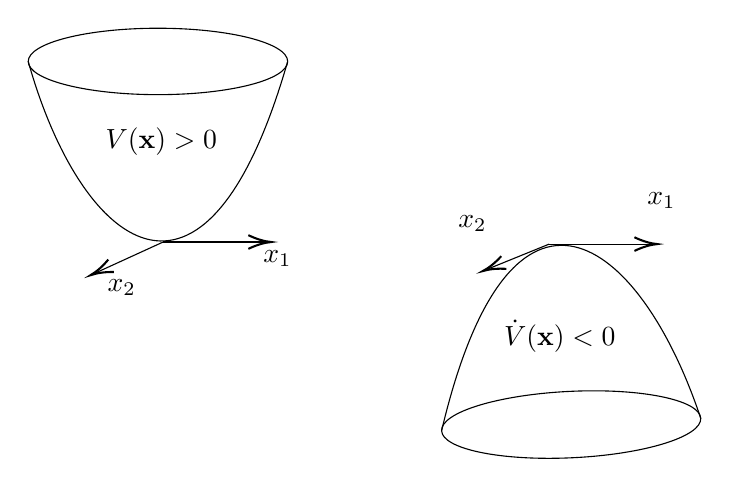
\begin{tikzpicture}[x=0.75pt,y=0.75pt,yscale=-1,xscale=1]
%uncomment if require: \path (0,300); %set diagram left start at 0, and has height of 300

%Curve Lines [id:da30536133686207734] 
\draw    (64,75.5) .. controls (89,164.5) and (149,214.5) .. (189,75.5) ;
%Shape: Ellipse [id:dp4415951216622267] 
\draw   (64,75.5) .. controls (64,66.66) and (91.98,59.5) .. (126.5,59.5) .. controls (161.02,59.5) and (189,66.66) .. (189,75.5) .. controls (189,84.34) and (161.02,91.5) .. (126.5,91.5) .. controls (91.98,91.5) and (64,84.34) .. (64,75.5) -- cycle ;
%Straight Lines [id:da051968201891894994] 
\draw    (129,162.5) -- (149,162.5) -- (179,162.5) ;
\draw [shift={(181,162.5)}, rotate = 180] [color={rgb, 255:red, 0; green, 0; blue, 0 }  ][line width=0.75]    (10.93,-3.29) .. controls (6.95,-1.4) and (3.31,-0.3) .. (0,0) .. controls (3.31,0.3) and (6.95,1.4) .. (10.93,3.29)   ;
%Straight Lines [id:da7438703353064577] 
\draw    (129,162.5) -- (95.82,177.67) ;
\draw [shift={(94,178.5)}, rotate = 335.43] [color={rgb, 255:red, 0; green, 0; blue, 0 }  ][line width=0.75]    (10.93,-3.29) .. controls (6.95,-1.4) and (3.31,-0.3) .. (0,0) .. controls (3.31,0.3) and (6.95,1.4) .. (10.93,3.29)   ;
%Curve Lines [id:da6434383410127575] 
\draw    (388.02,247.45) .. controls (358.77,159.75) and (296.44,112.69) .. (263.16,253.45) ;
%Shape: Ellipse [id:dp7059106277690401] 
\draw   (388.02,247.45) .. controls (388.44,256.28) and (360.83,264.78) .. (326.35,266.43) .. controls (291.88,268.09) and (263.58,262.27) .. (263.16,253.45) .. controls (262.74,244.62) and (290.34,236.12) .. (324.82,234.47) .. controls (359.3,232.81) and (387.59,238.62) .. (388.02,247.45) -- cycle ;
%Straight Lines [id:da45308326182855585] 
\draw    (315,163.5) -- (284.85,175.75) ;
\draw [shift={(283,176.5)}, rotate = 337.89] [color={rgb, 255:red, 0; green, 0; blue, 0 }  ][line width=0.75]    (10.93,-3.29) .. controls (6.95,-1.4) and (3.31,-0.3) .. (0,0) .. controls (3.31,0.3) and (6.95,1.4) .. (10.93,3.29)   ;
%Straight Lines [id:da2463038465244929] 
\draw    (315,163.5) -- (335,163.5) -- (365,163.5) ;
\draw [shift={(367,163.5)}, rotate = 180] [color={rgb, 255:red, 0; green, 0; blue, 0 }  ][line width=0.75]    (10.93,-3.29) .. controls (6.95,-1.4) and (3.31,-0.3) .. (0,0) .. controls (3.31,0.3) and (6.95,1.4) .. (10.93,3.29)   ;

% Text Node
\draw (100,106) node [anchor=north west][inner sep=0.75pt]   [align=left] {$\displaystyle V(\mathbf{x})  >0$};
% Text Node
\draw (292,199) node [anchor=north west][inner sep=0.75pt]   [align=left] {$\displaystyle \dot{V}(\mathbf{x}) < 0$};
% Text Node
\draw (176,165.4) node [anchor=north west][inner sep=0.75pt]    {$x_{1}$};
% Text Node
\draw (101,179.4) node [anchor=north west][inner sep=0.75pt]    {$x_{2}$};
% Text Node
\draw (361,137.4) node [anchor=north west][inner sep=0.75pt]    {$x_{1}$};
% Text Node
\draw (270,148.4) node [anchor=north west][inner sep=0.75pt]    {$x_{2}$};


\end{tikzpicture}


